\documentclass{standalone}
\usepackage{tikz}
\usetikzlibrary{patterns, positioning}


\begin{document}
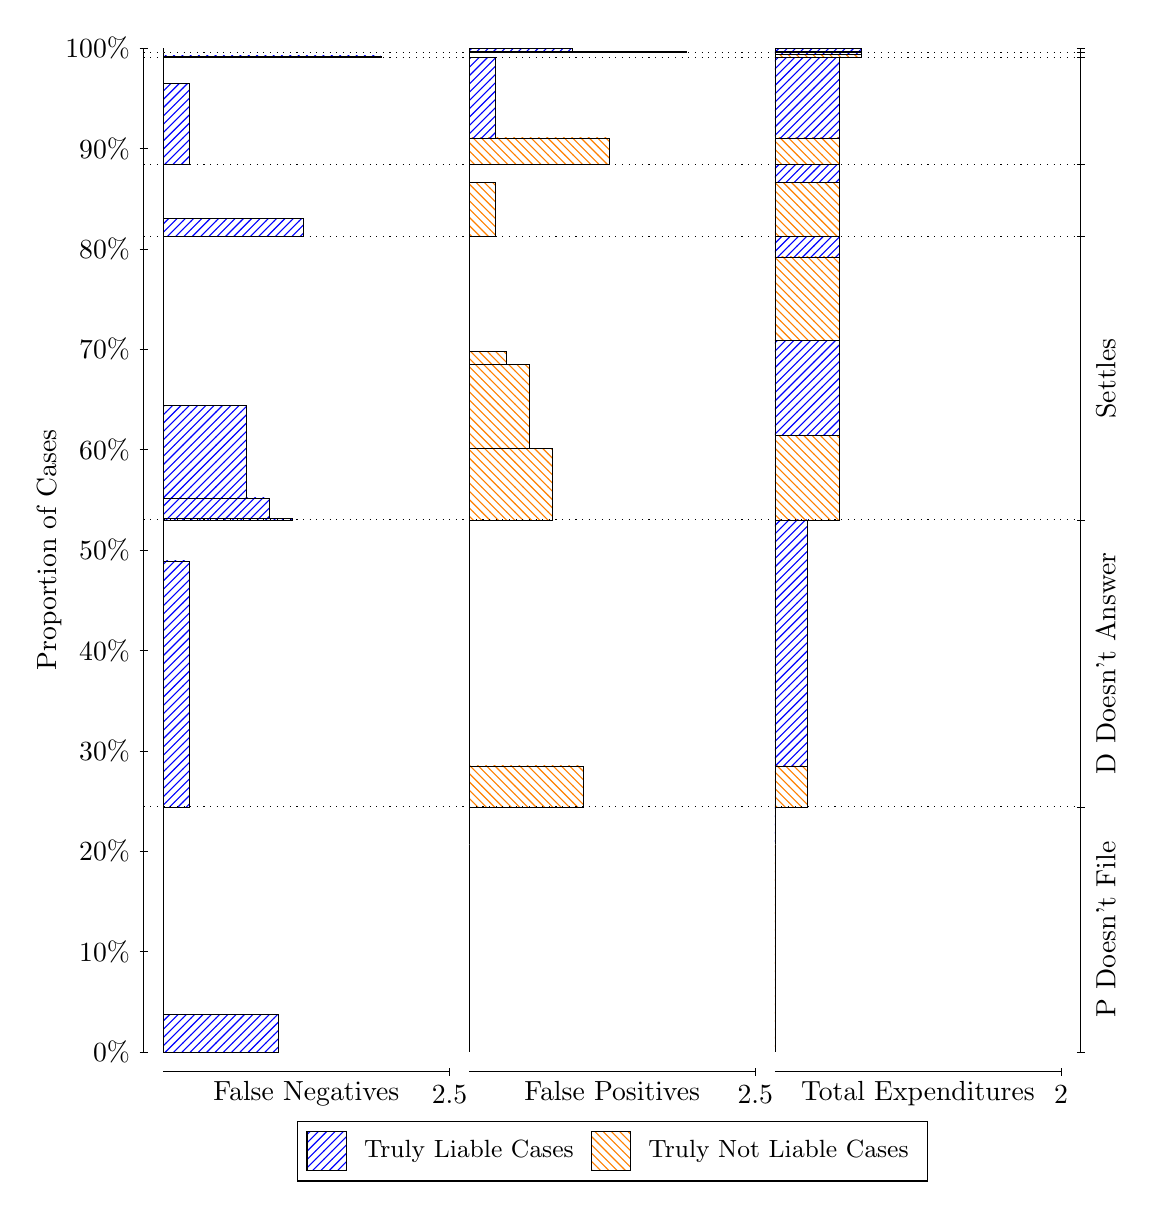
\begin{tikzpicture}
\draw[black, very thin] (1.5,1.75) -- (1.5,14.5);
\node[rotate=90, text=black, anchor=center] at (0.3, 8.125) {Proportion of Cases};
\draw[black, very thin] (1.45,1.75) -- (1.55,1.75);
\node[text=black, anchor=east] at (1.45, 1.75) {0\%};
\draw[black, very thin] (1.45,3.025) -- (1.55,3.025);
\node[text=black, anchor=east] at (1.45, 3.025) {10\%};
\draw[black, very thin] (1.45,4.3) -- (1.55,4.3);
\node[text=black, anchor=east] at (1.45, 4.3) {20\%};
\draw[black, very thin] (1.45,5.575) -- (1.55,5.575);
\node[text=black, anchor=east] at (1.45, 5.575) {30\%};
\draw[black, very thin] (1.45,6.85) -- (1.55,6.85);
\node[text=black, anchor=east] at (1.45, 6.85) {40\%};
\draw[black, very thin] (1.45,8.125) -- (1.55,8.125);
\node[text=black, anchor=east] at (1.45, 8.125) {50\%};
\draw[black, very thin] (1.45,9.4) -- (1.55,9.4);
\node[text=black, anchor=east] at (1.45, 9.4) {60\%};
\draw[black, very thin] (1.45,10.675) -- (1.55,10.675);
\node[text=black, anchor=east] at (1.45, 10.675) {70\%};
\draw[black, very thin] (1.45,11.95) -- (1.55,11.95);
\node[text=black, anchor=east] at (1.45, 11.95) {80\%};
\draw[black, very thin] (1.45,13.225) -- (1.55,13.225);
\node[text=black, anchor=east] at (1.45, 13.225) {90\%};
\draw[black, very thin] (1.45,14.5) -- (1.55,14.5);
\node[text=black, anchor=east] at (1.45, 14.5) {100\%};

\draw[black, very thin] (13.4,1.75) -- (13.4,14.5);
\draw[black, very thin] (13.35,1.75) -- (13.45,1.75);
\node[anchor=west] at (13.35, 1.75) {};
\draw[black, very thin] (13.35,4.8628) -- (13.45,4.8628);
\node[anchor=west] at (13.35, 4.8628) {};
\draw[black, very thin] (13.35,8.5083) -- (13.45,8.5083);
\node[anchor=west] at (13.35, 8.5083) {};
\draw[black, very thin] (13.35,12.103) -- (13.45,12.103);
\node[anchor=west] at (13.35, 12.103) {};
\draw[black, very thin] (13.35,13.025) -- (13.45,13.025);
\node[anchor=west] at (13.35, 13.025) {};
\draw[black, very thin] (13.35,14.379) -- (13.45,14.379);
\node[anchor=west] at (13.35, 14.379) {};
\draw[black, very thin] (13.35,14.443) -- (13.45,14.443);
\node[anchor=west] at (13.35, 14.443) {};
\draw[black, very thin] (13.35,14.5) -- (13.45,14.5);
\node[anchor=west] at (13.35, 14.5) {};

\draw[black, very thin, pattern color=blue, pattern=north east lines] (1.75,1.75) rectangle (3.2033,2.23);
\draw[black, very thin, pattern color=orange, pattern=north west lines] (1.75,2.23) rectangle (1.75,4.8628);
\draw[black, very thin, pattern color=blue, pattern=north east lines] (1.75,4.8628) rectangle (2.077,7.9868);
\draw[black, very thin, pattern color=orange, pattern=north west lines] (1.75,7.9868) rectangle (1.75,8.5083);
\draw[black, very thin, pattern color=blue, pattern=north east lines] (1.75,8.5083) rectangle (3.385,8.5314);
\draw[black, very thin, pattern color=blue, pattern=north east lines] (1.75,8.5314) rectangle (3.0943,8.7862);
\draw[black, very thin, pattern color=blue, pattern=north east lines] (1.75,8.7862) rectangle (2.8037,9.9663);
\draw[black, very thin, pattern color=orange, pattern=north west lines] (1.75,9.9663) rectangle (1.75,12.103);
\draw[black, very thin, pattern color=blue, pattern=north east lines] (1.75,12.103) rectangle (3.5303,12.338);
\draw[black, very thin, pattern color=orange, pattern=north west lines] (1.75,12.338) rectangle (1.75,13.025);
\draw[black, very thin, pattern color=blue, pattern=north east lines] (1.75,13.025) rectangle (2.077,14.046);
\draw[black, very thin, pattern color=orange, pattern=north west lines] (1.75,14.046) rectangle (1.75,14.379);
\draw[black, very thin, pattern color=blue, pattern=north east lines] (1.75,14.379) rectangle (4.5113,14.399);
\draw[black, very thin, pattern color=orange, pattern=north west lines] (1.75,14.399) rectangle (1.75,14.443);
\draw[black, very thin, pattern color=orange, pattern=north west lines] (1.75,14.443) rectangle (1.75,14.462);
\draw[black, very thin, pattern color=blue, pattern=north east lines] (1.75,14.462) rectangle (1.75,14.5);
\draw[black, very thin, pattern color=orange, pattern=north west lines] (5.6333,1.75) rectangle (5.6333,4.3828);
\draw[black, very thin, pattern color=blue, pattern=north east lines] (5.6333,4.3828) rectangle (5.6333,4.8628);
\draw[black, very thin, pattern color=orange, pattern=north west lines] (5.6333,4.8628) rectangle (7.0867,5.3842);
\draw[black, very thin, pattern color=blue, pattern=north east lines] (5.6333,5.3842) rectangle (5.6333,8.5083);
\draw[black, very thin, pattern color=orange, pattern=north west lines] (5.6333,8.5083) rectangle (6.687,9.4151);
\draw[black, very thin, pattern color=orange, pattern=north west lines] (5.6333,9.4151) rectangle (6.3963,10.478);
\draw[black, very thin, pattern color=orange, pattern=north west lines] (5.6333,10.478) rectangle (6.1057,10.645);
\draw[black, very thin, pattern color=blue, pattern=north east lines] (5.6333,10.645) rectangle (5.6333,12.103);
\draw[black, very thin, pattern color=orange, pattern=north west lines] (5.6333,12.103) rectangle (5.9603,12.79);
\draw[black, very thin, pattern color=blue, pattern=north east lines] (5.6333,12.79) rectangle (5.6333,13.025);
\draw[black, very thin, pattern color=orange, pattern=north west lines] (5.6333,13.025) rectangle (7.4137,13.359);
\draw[black, very thin, pattern color=blue, pattern=north east lines] (5.6333,13.359) rectangle (5.9603,14.379);
\draw[black, very thin, pattern color=orange, pattern=north west lines] (5.6333,14.379) rectangle (5.6333,14.424);
\draw[black, very thin, pattern color=blue, pattern=north east lines] (5.6333,14.424) rectangle (5.6333,14.443);
\draw[black, very thin, pattern color=orange, pattern=north west lines] (5.6333,14.443) rectangle (8.3947,14.462);
\draw[black, very thin, pattern color=blue, pattern=north east lines] (5.6333,14.462) rectangle (6.9413,14.5);
\draw[black, very thin, pattern color=orange, pattern=north west lines] (9.5167,1.75) rectangle (9.5167,4.3828);
\draw[black, very thin, pattern color=blue, pattern=north east lines] (9.5167,4.3828) rectangle (9.5167,4.8628);
\draw[black, very thin, pattern color=orange, pattern=north west lines] (9.5167,4.8628) rectangle (9.9254,5.3842);
\draw[black, very thin, pattern color=blue, pattern=north east lines] (9.5167,5.3842) rectangle (9.9254,8.5083);
\draw[black, very thin, pattern color=orange, pattern=north west lines] (9.5167,8.5083) rectangle (10.334,9.5815);
\draw[black, very thin, pattern color=blue, pattern=north east lines] (9.5167,9.5815) rectangle (10.334,10.785);
\draw[black, very thin, pattern color=orange, pattern=north west lines] (9.5167,10.785) rectangle (10.334,11.848);
\draw[black, very thin, pattern color=blue, pattern=north east lines] (9.5167,11.848) rectangle (10.334,12.103);
\draw[black, very thin, pattern color=orange, pattern=north west lines] (9.5167,12.103) rectangle (10.334,12.79);
\draw[black, very thin, pattern color=blue, pattern=north east lines] (9.5167,12.79) rectangle (10.334,13.025);
\draw[black, very thin, pattern color=orange, pattern=north west lines] (9.5167,13.025) rectangle (10.334,13.359);
\draw[black, very thin, pattern color=blue, pattern=north east lines] (9.5167,13.359) rectangle (10.334,14.379);
\draw[black, very thin, pattern color=orange, pattern=north west lines] (9.5167,14.379) rectangle (10.607,14.424);
\draw[black, very thin, pattern color=blue, pattern=north east lines] (9.5167,14.424) rectangle (10.607,14.443);
\draw[black, very thin, pattern color=orange, pattern=north west lines] (9.5167,14.443) rectangle (10.607,14.462);
\draw[black, very thin, pattern color=blue, pattern=north east lines] (9.5167,14.462) rectangle (10.607,14.5);
\draw[black, dotted] (1.5,4.8628) -- (13.4,4.8628);
\draw[black, dotted] (1.5,8.5083) -- (13.4,8.5083);
\draw[black, dotted] (1.5,12.103) -- (13.4,12.103);
\draw[black, dotted] (1.5,13.025) -- (13.4,13.025);
\draw[black, dotted] (1.5,14.379) -- (13.4,14.379);
\draw[black, dotted] (1.5,14.443) -- (13.4,14.443);
\draw[black, very thin] (1.75,1.5) -- (5.3833,1.5);
\node[text=black, anchor=north] at (3.5667, 1.5) {False Negatives};
\draw[black, very thin] (5.3833,1.45) -- (5.3833,1.55);
\node[text=black, anchor=north] at (5.3833, 1.45) {2.5};

\draw[black, very thin] (5.6333,1.5) -- (9.2667,1.5);
\node[text=black, anchor=north] at (7.45, 1.5) {False Positives};
\draw[black, very thin] (9.2667,1.45) -- (9.2667,1.55);
\node[text=black, anchor=north] at (9.2667, 1.45) {2.5};

\draw[black, very thin] (9.5167,1.5) -- (13.15,1.5);
\node[text=black, anchor=north] at (11.333, 1.5) {Total Expenditures};
\draw[black, very thin] (13.15,1.45) -- (13.15,1.55);
\node[text=black, anchor=north] at (13.15, 1.45) {2};

\node[text=black, centered, rotate=90] at (13.72, 3.3064) {P Doesn't File};
\node[text=black, centered, rotate=90] at (13.72, 6.6855) {D Doesn't Answer};
\node[text=black, centered, rotate=90] at (13.72, 10.305) {Settles};





\draw (7.449999999999999,1.5) node[draw=none] (baseCoordinate) {};
\begin{scope}[align=center]
        \matrix[scale=0.5, draw=black, below=0.5cm of baseCoordinate, nodes={draw}, column sep=0.1cm]{
            \node[rectangle, draw, minimum width=0.5cm, minimum height=0.5cm, pattern color=blue, pattern=north east lines] {}; &
            \node[draw=none, font=\small, text=black] (B) {Truly Liable Cases}; &
            \node[rectangle, draw, minimum width=0.5cm, minimum height=0.5cm, pattern color=orange, pattern=north west lines] {}; &
            \node[draw=none, font=\small, text=black] (B) {Truly Not Liable Cases}; \\
            };
\end{scope}

\end{tikzpicture}
\end{document}